\documentclass[10pt, a4paper,spanish]{article}

\usepackage[utf8]{inputenc}
\usepackage[spanish]{babel}

\usepackage[T1]{fontenc}

\usepackage[hmarginratio=1:1,top=32mm,columnsep=20pt]{geometry}
\usepackage[hang, small,labelfont=bf,up,textfont=it,up]{caption}

\usepackage{float}

\usepackage{graphicx}
\graphicspath{ {images/} }

\usepackage{titlesec}
\renewcommand\thesection{\Roman{section}}
\renewcommand\thesubsection{\Roman{subsection}}
\titleformat{\section}[block]{\large\scshape\centering}{\thesection.}{1em}{}
\titleformat{\subsection}[block]{\large}{\thesubsection.}{1em}{}

\usepackage{fancyhdr}
\pagestyle{fancy}
\fancyhead{}
\fancyfoot{}
\fancyhead[C]{ \today \ $\bullet$ Ingeniería del Conocimiento $\bullet$ Sistemas Basados en Reglas}
\fancyfoot[RO]{\thepage}

%-------------------------------------------------------------------------------
%	TITLE SECTION
%-------------------------------------------------------------------------------

\title{\vspace{-15mm}\fontsize{24pt}{10pt}\selectfont\textbf{Sistemas Basados en Reglas}} % Article title

\author{Sergio García Prado}
\date{\today}

%-------------------------------------------------------------------------------

\begin{document}

	\maketitle % Insert title

	\thispagestyle{fancy} % All pages have headers and footers

%-------------------------------------------------------------------------------
%	TEXT
%-------------------------------------------------------------------------------

	\begin{figure}[H]
		\begin{center}
			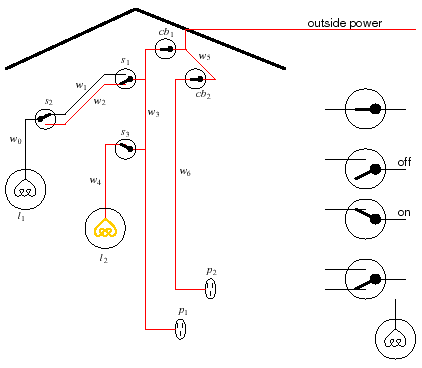
\includegraphics[width=0.6\textwidth]{diagnostic-assistant}
		\end{center}
	\end{figure}


	\section{Desarrollar una base de conocimiento para la versión reducida del asistente al diagnóstico que muestra la figura. Utilizar un lenguaje de tripletes O-A-V, permitiendo el uso de variables en las reglas para los Objetos y los Valores}

		\paragraph{}


	\section{Obtener la red RETE que genera el siguiente conjunto de reglas}

	\begin{figure}[H]
		\begin{center}
			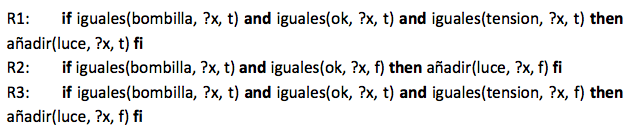
\includegraphics[width=0.8\textwidth]{rete-exercise}
		\end{center}
	\end{figure}

\end{document}
